%# -*- coding: utf-8 -*-
% !TEX encoding = UTF-8 Unicode
\RequirePackage{fixltx2e}
\documentclass[aps,pre,12pt,preprint,onecolumn,showpacs,showkeys,UTF8]{revtex4-1}
\usepackage{ctex}
\usepackage{mathrsfs}
\usepackage{setspace,dcolumn}
\usepackage{subfigure}
\usepackage{graphicx,psfrag,epsfig}
\usepackage[font=small,format=plain,labelfont=bf,textfont=it,justification=raggedright,singlelinecheck=false]{caption}
\usepackage{amsmath,amsfonts,amssymb,amsthm,bm,upgreek}
\usepackage{geometry}
\usepackage[mathscr]{eucal}
\usepackage{titlesec}
\usepackage{tabularx}
\titleformat{\section}{\bf\fangsong\zihao{4}}{\thesection}{0.75em}{}
\geometry{top=2.54cm,bottom=2.54cm,left=3cm,right=3cm}
\renewcommand\appendixname{附录}
\renewcommand\abstractname{}%摘要
\renewcommand\tablename{表}
\renewcommand\figurename{图}
\makeatletter
\def\@keys@name{\songti\zihao{-4}{\bf 关键词:}}
\def\Received@name{\zihao{-5}{接收} }
\def\Revised@name{\zihao{-5}{修订} }
\def\Accepted@name{\zihao{-5}{采纳} }
\def\Published@name{\zihao{-4}{发表} }
\makeatother
\linespread{1.6}
\renewcommand{\labelenumi}{\alph{enumi}.}
\leftmargini=20mm

\begin{document}

\title{\bf\heiti\zihao{3}钠原子光谱的观测与研究\vspace{15mm}}
\author{\fangsong 乔颢\vspace{2mm}}
\affiliation{\songti\zihao{-4}北京大学物理学院2011级2班~~~~学号:1100011354 \vspace{2mm}}
\keywords{钠原子光谱, 精细结构, 能级图, 量子缺}
\email{1993422qsh@gmail.com; 18600200672}
\begin{abstract}
	\vspace{10mm}
	\begin{spacing}{1.5}
		\songti\zihao{-4}
		本实验利用光栅光谱仪,对钠原子的光谱进行了详细的测量。通过对钠原子光谱中双线结构的具体分析,计算出来了钠原子不同线系的量子缺,分别为主线系0.892,漫线系0.008,锐线系1.349。同时得到了钠原子的3P轨道有效电荷数为3.586。
	\end{spacing}
\end{abstract}

\maketitle

\section{引言}
对元素的光谱进行研究是了解原子结构的重要途径之一。通过对于氢原子的光谱的研究,人们认识到了电子在围绕原子核运动时轨道是分立的。而对于钠原子则是一个多电子系统,对于钠原子的光谱的研究,使得人们更于清晰的了解了碱金属的电子层级结构。本实验通过对于钠原子光谱的研究,计算出钠原子价电子的量子缺,绘制出部分能级图,并且根据双线波长差计算价电子运动的时候电子实的有效电荷。

氢原子的光谱中波数可以用一下公式表示:
\begin{equation}
	\tilde{v}=\frac{R}{n_2^2}-\frac{R}{n_1^2}
\end{equation}
而对于碱原子来说,内层电子和原子核形成了原子实,所以实际上对于外层电子影响的电荷量和轨道有关。当主量子数不大的时候,这个只和角量子数有关,表述如下:
\begin{equation}
	T_{nl}=\frac{(Z_n^*)R}{n^2}=\frac{R}{(n-\Delta_l)^2}
\end{equation}

因为自旋轨道耦合,能级出现了分裂,这里也就是精细结构的出现,从理论上可以推出,对于量子数为n,l,j的能级,$j=|l\pm\frac{1}{2}|$。 有
\begin{equation}
	T_{n,l,j=l+1/2}=\frac{R}{(n'-\Delta_l')^2}-\frac{l}{2}\xi_{n,l}
\end{equation}
\begin{equation}
	T_{n,l,j=l-1/2}=\frac{R}{(n'-\Delta_l')^2}+\frac{l+1}{2}\xi_{n,l}
\end{equation}
其中有$\xi_{n,l}=\frac{R \alpha^2(Z^*)^4}{n^3l(l+1/2)(l+1)}$,所以能级分裂,波数差为:
\begin{equation}
	\Delta \tilde{v}=(l+1/2)\xi_{n,l}=\frac{R\alpha^2(Z^*)^4}{n^3l(l+1)}
\end{equation}

同时能级跃迁时候发射的光谱线强度可以由以下公式确认:
\begin{equation}
	I_{nm}=N_nA_{nm}hv_{nm}
\end{equation}
所以根据谱线跃迁的强度和定则,可以得到,对于主线系,$\frac{I_{PA}}{I_{PB}}=\frac{g_{3/2}}{g_{1/2}}=\frac{2}{1}$。锐线系有:$\frac{I_{SA}}{I_{SB}}=\frac{1}{2}$,漫线系有$\frac{I_{DA}}{I_{DB}}=\frac{1}{2}$。

这次实验通过对于钠原子光谱的探测,了解钠原子光谱的规律和其产生的原因,同时熟悉光栅光谱仪的使用。

\section{实验}
\subsection{实验装置}
\begin{enumerate}
	\item 光谱仪\ 国产WGD-8A型多功能光栅光谱仪以及其配套软件。
	\item 光源\ GY-5 钠光灯。
\end{enumerate}
\subsection{实验步骤以及数据}
打开计算机,打开仪器以及钠光灯,并对其进行预热。在系统稳定前光谱线可能不是很稳定。等到整体系统稳定后,可以进行仪器的测试以及校准。

首先将入射光阑和出射光阑都调整到合适的位置(大概不大不小),增益的负高压都调整为1,这时进行一次全谱的预扫描,来检测仪器是否正常工作。可以观测到输出的光谱强度图像在590nm左右出现极大,这也就是钠双黄线,本次实验要据此对光谱仪进行校准工作。

调整扫描范围在双黄线对应的位置,然后减少入射光强,对双黄线光谱进行详细的扫描。在光强增益调整合适的情况下测峰得到对应的钠双黄线的波长,与理论值比较后输入相对差值来校准仪器。校准过后仪器给出的波长就应该是正确的波长值。截图如下。此时测量的参数为:增益1,电压330V,负高压1,入射狭缝读数3.784mm,出射读数3.442mm。

\begin{figure}[h]
	\begin{center}
		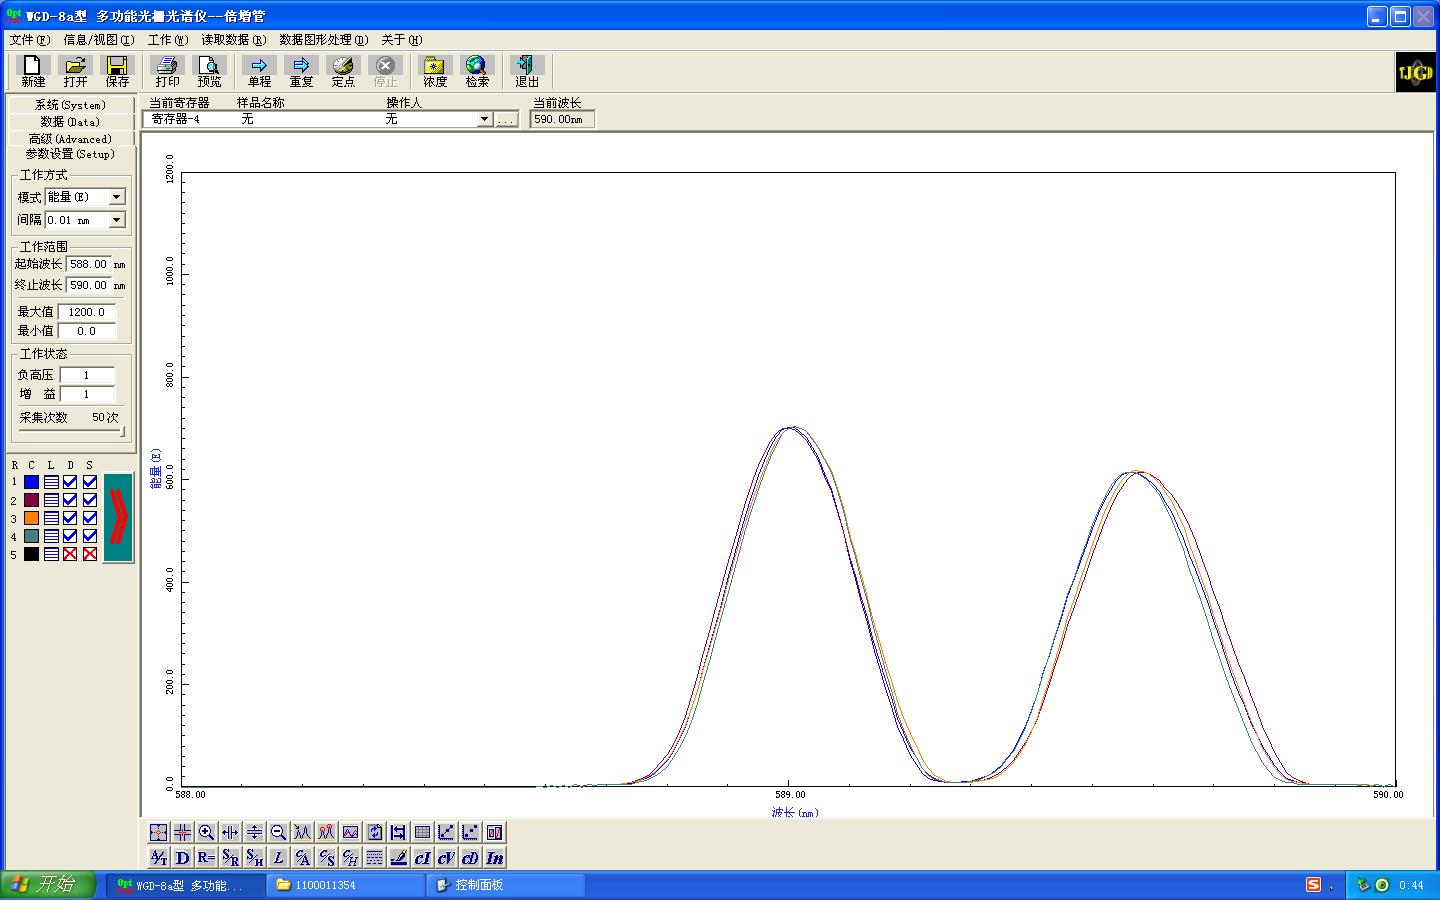
\includegraphics[width=0.7\textwidth]{pic1.png}
		\caption{\label{fig:exp1}校准后钠双黄线的强度和波长关系图}
	\end{center}
\end{figure}

\newpage

随后可以细致扫描全谱,此时的光强应该偏大,然后在光谱强度图中寻找有波动的地方,并对其进行更为精细的扫描得到具体的光谱。在调整过程中,调节入射光阑影响的是光强以及波峰的半高宽,所以如果发现两个波峰无法分开的时候可以将入射光阑调小。出射光阑影响分光后对光线接受的范围,其直接影响光的强弱,但是采集器实际上测量的是出射光阑范围内所有的光强和,所以当出射光阑过大会造成图案的畸变。增益则是整体放大输入信号的,可以配合负高压调整整个图像的质量。

对测量得到的波峰进行计算比较可以得到双峰的具体分布情况,如表\ref{table1}:
\begin{center}
	\begin{table}
		\caption{全谱扫描具体峰的参数}
		\label{table1}
		\begin{tabular}{cccccc}
			\hline
			\hline
			波长/nm&峰值&负高压&增益&入射狭缝/mm&出射狭缝/mm \\
			\hline
			330.12&&3&3&0.375&2.001\\
			\hline
			416.39&396.8&1&2&2.78&2.93\\
			417.01&47.1\\
			\hline
			419.61&221.0&3&6&2.20&2.83\\
			420.33&229.0\\
			420.56&639.8\\
			\hline
			425.68&30.8&3&3&2.38&2.83\\
			426.49&190.1\\
			427.18&137.1\\
			427.72&223.3\\
			430.46&168.1\\
			\hline
			433.39&131.6&3&6&2.20&2.79\\
			434.12&50.8\\
			435.04&69.9\\
			436.29&45.5\\
			\hline
			451.52&150.7&3&6&2.42&2.79\\
			452.61&57.0\\
			\hline
			466.93&86.2&1&6&2.42&2.90\\
			467.28&162.6\\
			470.64&147.5\\
			\hline
			498.32&207.1&1&3&2.42&2.90\\
			498.73&400.0\\
			\hline
			515.27&111.4&1&6&2.42&2.90\\
			515.70&217.6\\
			516.54&65.0\\
			519.09&85.2\\
			\hline
			545.64&47.6&1&6&2.42&2.90\\
			546.50&107.7\\
			549.80&123.5\\
			556.17&125.3\\
			557.47&45.4\\
			561.06&132.6\\
			\hline
			568.46&434.1&1&1&2.35&2.90\\
			569.10&861.0\\
			\hline
			589.00&348.4&1&1&2.12&2.90\\
			589.57&306.9\\
			\hline
			581.56&49.4&1&1&2.42&2.90\\
			\hline
			603.37&278.4&1&6&2.42&2.90\\
			604.42&105.7\\
			\hline
			615.37&326.0&1&4&2.42&2.90\\
			616.10&644.9&1&4&2.42&2.90\\
			\hline
			\hline
		\end{tabular}
	\end{table}
\end{center}

从数据表中可以看出不少双峰的数据,当然还有很多其他的数据,这些数据可能来自于钠灯的杂质等等。对数据进行整理可以找出各线系的谱线:

主线系谱线:
\begin{enumerate}
	\item 波长位于330.12nm,双峰不可分辩,能级为3S-4P。
	\item 波长位于589.28nm,双峰强度比1.14,能级为3S-3P。
	\item 查表计算可得a=0.108,$\Delta_l$=0.892。
\end{enumerate}

漫线系谱线:
\begin{enumerate}
	\item 波长位于467.10nm,双峰强度比0.53,能级为3P-6D。
	\item 波长位于498.52nm,双峰强度比0.52,能级为3P-5D。
	\item 波长位于568.78nm,双峰强度比0.50,能级位3P-4D。
	\item 查表计算可得a=0.989,0.995,$\Delta_l$=0.011,0.005。
\end{enumerate}

锐线系谱线:
\begin{enumerate}
	\item 波长为515.48nm,双峰强度比为0.51,能级为3P-6S。
	\item 波长为615.74nm,双峰强度比为0.50,能级为3P-5S。
	\item 查表计算可得a=0.651,$Delta_l$=1.349。
\end{enumerate}

最后可以计算出对应的量子缺以及固定项目,如表\ref{table2}:
\begin{center}
	\begin{table}
		\caption{各线系量子缺和固定项}
		\label{table2}
		\begin{tabular}{m{4cm}<{\centering}m{4cm}<{\centering}m{4cm}<{\centering}}
			\hline
			\hline
			线系&量子缺&固定项/$cm^{-1}$\\
			\hline
			主线系&0.892&41652.4\\
			漫线系&0.008&24463.0\\
			锐线系&1.349&24472.0\\
			\hline
			\hline
		\end{tabular}
	\end{table}
\end{center}

做出来的能级图,如图\ref{fig:exp1}:
\begin{figure}[h]
	\begin{center}
		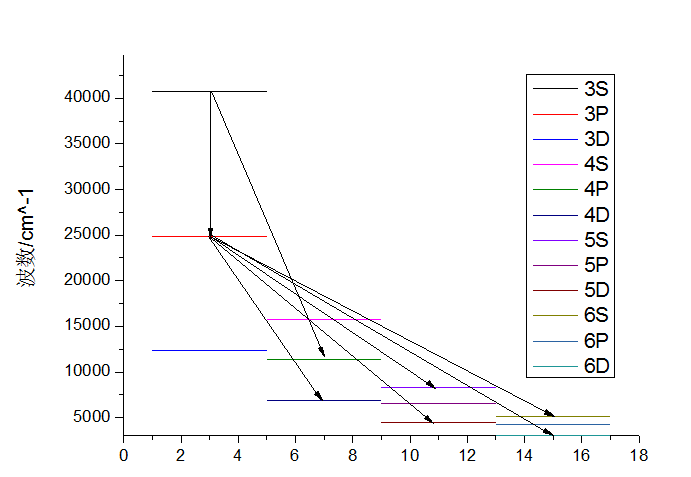
\includegraphics[width=0.7\textwidth]{pic2.png}
		\caption{\label{fig:exp1}钠原子光谱图。}
	\end{center}
\end{figure}

共振线和锐线系的平均波数差为17.72$cm^{-1}$。对应的有效电荷数为$Z_s^*=3.586$。


\section{结论}

本次实验利用光栅光谱仪测量得到了钠原子光谱的一些性质,做出了钠原子的光谱图\ref{fig:exp1},计算出了主线系的量子缺为0.892,漫线系为0.008,锐线系为1.349。以及3P轨道的有效电荷数为3.586。

\section{致谢} 
感谢赵子强老师的指导,以及贾春燕,冉书能老师的技术支持。


\begin{thebibliography}{}
	\bibitem{Book} 吴思成,王祖铨~2010 近代物理实验(第三版)(北京:高等教育出版社)第17页.%
%
\end{thebibliography}

\clearpage
\appendix
\section{思考题}
1、照明光路仪器基本提供,需要注意的就是光源要贴近如射光阑防止其他杂光的入射。

2、通过仪器进行全谱的检测,然后找到钠双黄线,将其与标准值做对比然后对仪器进行校准即可。测量光谱线的波长只需合适的调整增益以及光阑,使得仪器探测到良好的高斯峰,然后对应的高斯峰峰值波长就是谱线的波长。

3、正如上文所说的,调整入射光阑决定了光强(峰的高度)以及分辨率(峰的宽度)。所以在分不清楚两个峰的时候应该减少入射光阑。出射光阑则会影响探测的光强(峰的高度)和效果(图像的畸变)。如果遇到了峰不像是高斯峰的样子则可以调整出射光阑。而增益和负高压等也影响了整体图像的质量。总之在能探测到合适强度的光波的时候尽量增加分辨率并且保持图片的完整是最后的目的。

4、根据双峰的风高就可以判断出主线系,然后通过峰的尖锐程度可以初步判断锐线系和漫线系。

5、不是完全的一致。可能因为光源的温度以及仪器自身的精度导致实验的结果有一定的上下波动,同时因为增益的问题会引入底躁,从而使得谱线的高度收到了相当的影响。

\section{记录本}
已经检查了,就不上传了。

\end{document} 
